\section{Analysis}

\subsection{What trends, correlations, and/or patterns do you see in the data?}

Different trends were observed for different data. This section will outline the results of our analysis for the three crops.

\subsubsection{Poultry}

The data frame used for the final analysis contained eight observations.
When the prices and production were plotted using a scatterplot, a clear linear relationship was observed.
The scatterplot and trend-line for this relationship can be observed in Figure~\ref{fig:chicken_scatter}.
Using the statsmodels package in Python, we determined the coefficients for the linear model using the ordinary least squares (OLS) approach.
The output from the regression can be viewed in Figure~\ref{fig:chicken_ols}.

\begin{figure}
    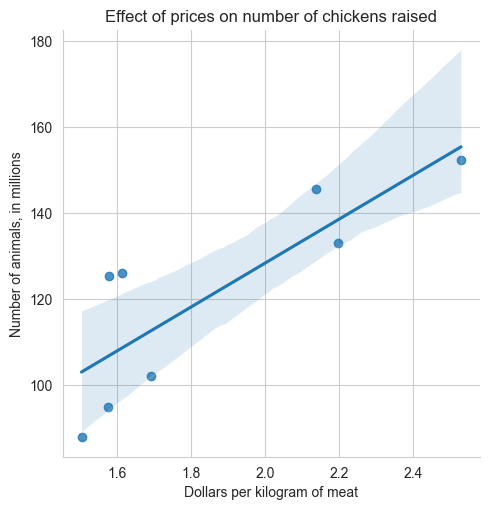
\includegraphics[width=\linewidth]{chicken_scatter}
    \caption{A scatter plot of chicken prices vs. chicken production.}
    \label{fig:chicken_scatter}
\end{figure}

The null hypothesis for this test was that no relationship exists between price and production.
Following the regression, there was the resulting model:

\\~\\

\tabto{5cm} $y = 26.4810 + 50.9459x_1$


\begin{itemize}
    \item Where $y$ is the price of chicken meat, in dollars per kilogram
    \item and $x_1$ is the number of chickens, measured in millions of individuals
\end{itemize}

\begin{figure}
    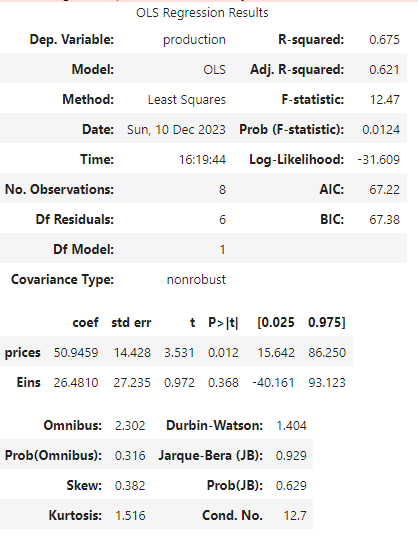
\includegraphics[width=\linewidth]{chicken_ols_results}
    \caption{Results from an Ordinary Least Squares Regression.}
    \label{fig:chicken_ols}
\end{figure}

The F-statistic for this model was observed to be $12.47$; under a normal distribution the chances of observing this value are $~0.01\%$.
Setting our p-value to $0.05$, we would be forced to reject the null hypothesis and conclude there is indeed a relationship between the price and production of chicken in Canada.
Finally, The observed value for $R^2$ was $0.675$ which means that approximately 67\% of the variance of the data can be accounted for by this model.

\subsubsection{Hog}

\subsubsection{Wheat}



